\subsection{T0 and BHD analysis}
T0 is the time reference detector for all data located downstream of the D5 magnet.
BHD is a detector located approximately 7.7 m upstream and confirms that the beam particles are in fact Kaon by the T0-BHD TOF method.
The multiplicity of T0 and BHD in an unbiased kaon trigger is shown in Fig.\ref{fig:BHDT0_mul}.
T0 requires one hit to be the reference for all, whereas BHD is installed upstream and has many events with more than one hit.
In order to increase the number of events that can be analysed, events are not selected by the number of hits in the BHD.
\begin{figure}
  \begin{tabular}{cc}
    \begin{minipage}{0.5\hsize}
      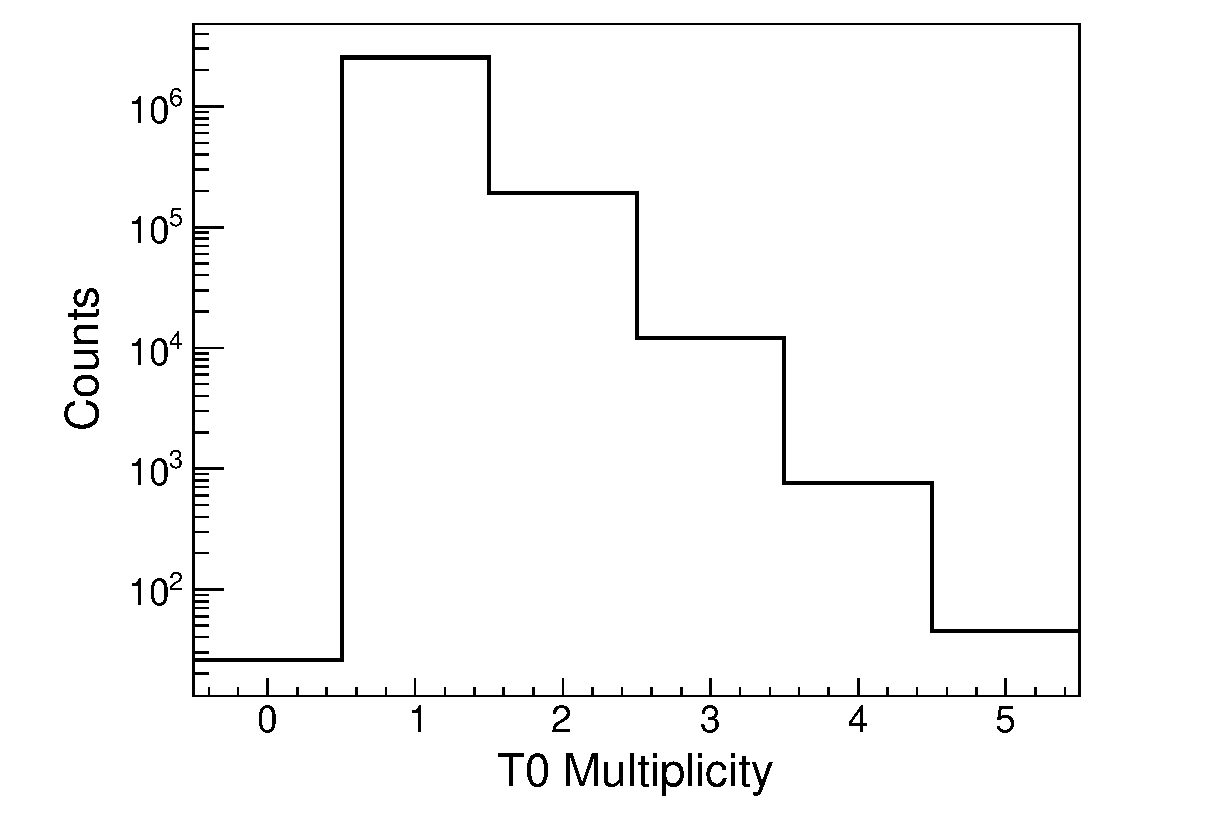
\includegraphics[width=5cm]{../pic/Run78/BL/nT0.eps}
    \end{minipage}

    \begin{minipage}{0.5\hsize}
      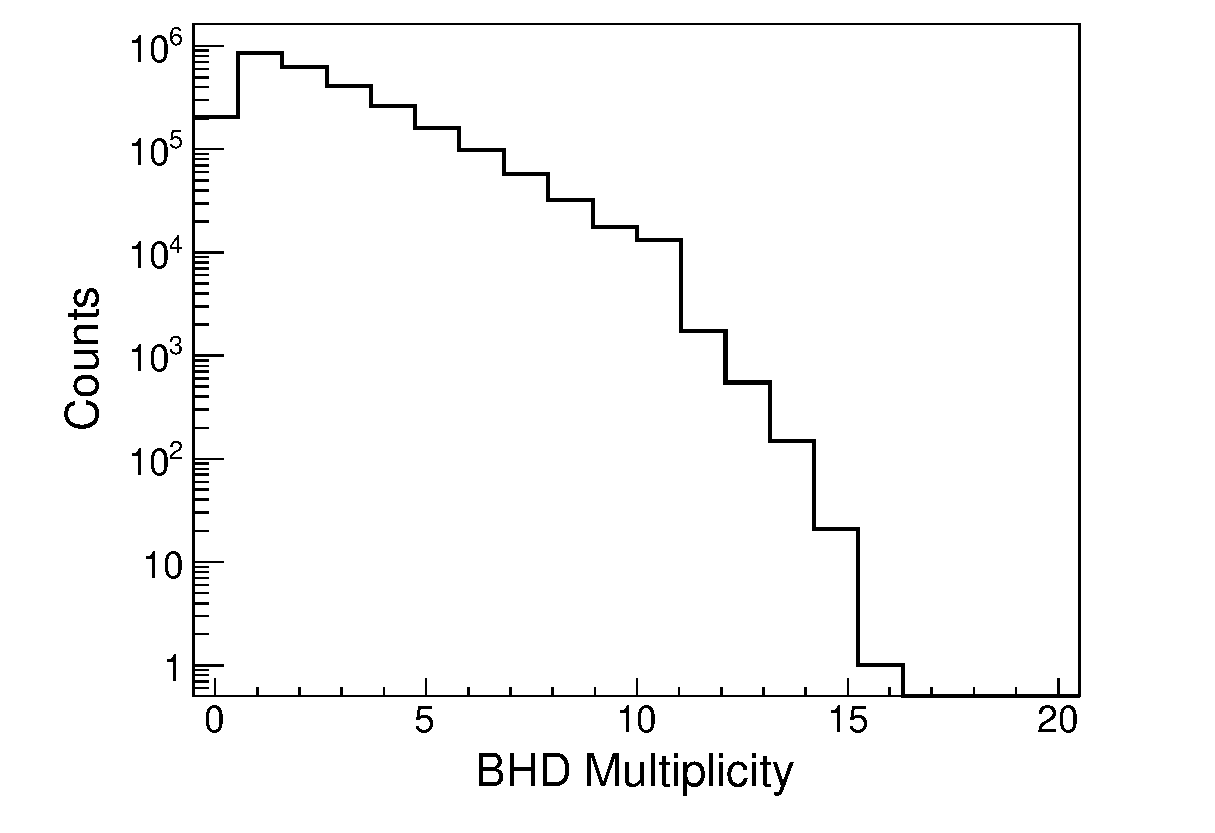
\includegraphics[width=5cm]{../pic/Run78/BL/nBHD.eps}
    \end{minipage}
  \end{tabular}
  \caption{
    These figures show T0 and BHD multiplicity on a log scale.
    The left and right figures are for T0 and BHD respectively.
  }
  \label{fig:BHDT0_mul}
\end{figure}


Fig.\ref{fig:BHDT0_TOF} represents the BHD-T0 time-of-flight (TOF) with unbiased Kaon triggering. All BHD hit combinations are plotted.
Two peaks are seen around 29ns and 26ns, which correspond to $1$GeV$/c$ pion and kaon flight times at 7.7m.
The kaon peaks are fitted with a Gaussian and the acceptable region for kaon events is determined by 3 sigma, this is represented by the area hatched in red.

\begin{figure}
  \centering
  \includegraphics[width=7cm]{../pic/Run78/BL/BHDT0_TOF.eps}
  \caption{
    BHD-T0 time-of-flight with 7.7m flight length on a log scale.
    The red hatched plot indicates an acceptable reigion as a kaon.
  }
  \label{fig:BHDT0_TOF}
\end{figure}

